\section*{Methods}

\subsection*{Ocean reanalyses}

Three reanalyses are computed here from monthly fields (Extended Data
Table~1). ORAS5\cite{Zuo2019} is a NEMO configuration at 0.25\degree{} with 75
vertical levels, assimilated by NEMOVAR 3D-Var FGAT and forced by ERA-40,
ERA-Interim and ERA5; we use 816 gap-free monthly fields of meridional velocity
and salinity covering 1958--2025. The Copernicus distribution joins the
consolidated reanalysis, which ends in 2014, to the operational stream
thereafter, and the two are treated separately wherever it matters.
GLORYS12V1\cite{JeanMichel2021} is a NEMO configuration at 1/12\degree{} with 50
levels, assimilated by a reduced-order Kalman filter and forced by ERA-Interim
and ERA5; we use 396 monthly fields covering 1993--2025. ECCO-V4r4\cite{Forget2015}
is an MITgcm state estimate on the LLC90 grid, nominally 1\degree{}, fitted to
observations by the adjoint method and therefore dynamically consistent by
construction, with no assimilation increments; its atmospheric forcing is
ERA-Interim plus estimated control adjustments. We analyse the distributed
0.5\degree{} lat-lon interpolation with 50 levels, using all 312 monthly fields
covering 1992--2017. Interpolation from the native grid does not conserve volume
transport exactly, which is a limitation we state rather than correct.

SODA 3.15.2\cite{Carton2018} is shown in Fig.~\ref{fig:sign}a for context but is
not used in any quantitative claim. It is a MOM5 and SIS configuration run at
1/4\degree{}, assimilated by optimal interpolation with bias correction and
forced by ERA5, and the archive we can obtain provides annual rather than
monthly fields on a regridded 0.5\degree{} Mercator grid. Because $\Fovs$ is
bilinear in velocity and salinity, forming it from annual means omits the
within-year covariance; measured in ECCO, where both routes are available, the
omission shifts $\Fovs$ by $+0.0124$~Sv, exceeding SODA's record mean of
$-0.0091$~Sv in magnitude. The corresponding shifts are $+0.0000$~Sv in ORAS5
and $-0.0013$~Sv in GLORYS12V1.

\subsection*{The section}

At the grid row nearest 34.5\degS{},
\begin{equation}
\Fovs \;=\; -\frac{1}{S_0}\int_{-H}^{0} V_{bc}(z)\,\big[\bar{S}(z)-S_0\big]\,\mathrm{d}z,
\label{eq:fovs}
\end{equation}
where $V_{bc}(z)$ is the zonally integrated meridional velocity after removal of
the net section transport, $\bar{S}(z)$ the width-weighted zonally averaged
salinity and $S_0=35$~PSU. A negative $\Fovs$ means the overturning imports
freshwater, equivalently that it exports salt from the Atlantic.

The Atlantic segment at each row is the contiguous run of ocean points
containing 25\degW{}, rather than a fixed longitude box. This matters. A box
from 70\degW{} to 20\degE{} at 34.5\degS{} admits, in GLORYS12V1, a second water
body of about 20 grid points near 58 to 57\degW{} whose surface salinity is
0.00 to 0.04~PSU. Those values are too fresh for the outer R\'io de la Plata,
which is brackish rather than fresh, so they are most likely estuary, lake or
land-mask cells rather than a resolved plume; either way they are not part of the
open Atlantic along this row. Including them depresses $\bar{S}$ in the upper
cells and shifts $\Fovs$ by $+0.013$~Sv, about a sixth of the GLORYS12V1 record
mean. At the 0.5\degree{} resolution of ECCO the feature is unresolved and the
contiguity test makes no difference. The resulting sections contain 294 ocean
points at 34.56\degS{} in ORAS5, 881 at 34.50\degS{} in GLORYS12V1 and 146 at
34.75\degS{} in ECCO; these are counts of ocean points, not of the width of a
longitude box.

The net transport removed is $-1.22$~Sv in ORAS5, $-1.17$ in GLORYS12V1 and
$-0.98$ in ECCO, and removing it shifts $\Fovs$ by $+0.0086$, $+0.0083$ and
$+0.0066$~Sv. It is of the sign and order expected for the Bering Strait inflow
plus net precipitation minus evaporation over the basin to the north, but we do
not claim it is that quantity: across the latitude ladder it varies
non-monotonically by 1.1~Sv in ORAS5 and 2.5~Sv in GLORYS12V1, far more than the
precipitation minus evaporation of the intervening bands, so a substantial part
of it is section construction, grid metrics or genuine mass imbalance. The
justification for removing it is that an overturning component of the freshwater
transport is not defined without doing so, and that equation~\eqref{eq:fovs} is
otherwise sensitive to $S_0$.

The azonal component is
$F_{az}=-(1/S_0)\iint v'S'\,\mathrm{d}x\,\mathrm{d}z$, with primes the
departures from the width-weighted zonal mean at each depth. It is computed from
monthly means and therefore excludes sub-monthly covariance.

\subsection*{The limb factorisation}

Because $\int V_{bc}\,\mathrm{d}z=0$, the depth levels where $V_{bc}>0$ carry a
volume transport $T$ exactly balanced by $-T$ in the levels where $V_{bc}<0$.
Defining the transport-weighted limb salinities
\begin{equation}
S_{\uparrow}=\frac{1}{T}\int_{V_{bc}>0}\! V_{bc}\bar{S}\,\mathrm{d}z,
\qquad
S_{\downarrow}=\frac{1}{T}\int_{V_{bc}<0}\! (-V_{bc})\bar{S}\,\mathrm{d}z,
\end{equation}
equation~\eqref{eq:fovs} becomes $\Fovs=-T(S_{\uparrow}-S_{\downarrow})/S_0$
exactly, because the $-S_0$ term integrates to zero. Both factors are computed
directly from the section profile and neither is defined in terms of the other,
which is what distinguishes this from writing $\Fovs=-\Psi\,\Delta_v S/S_0$
with $\Delta_v S\equiv-S_0\Fovs/\Psi$. In that construction the second factor is
the first divided out; it absorbs every change in the vertical structure of the
velocity as well as every change in salinity, it closes to machine precision by
construction, and the implied overturning share is fixed by the algebraic
identity
$(\Psi\text{ term})/\Delta\Fovs=(F_{\mathrm{early}}/\Delta\Fovs)\,(\delta\Psi/\Psi_{\mathrm{early}})$,
where $F_{\mathrm{early}}$ and $\Psi_{\mathrm{early}}$ are the base-epoch
values. We do not use it except as a labelled sensitivity test, and we note that
because that construction pins the share to the ratio of fractional changes it
cannot return a large value whatever the physics. The residual of the limb
factorisation is below $1.5\times10^{-14}$~Sv, which is double-precision
round-off and confirms only that the net transport removal closed.

\subsection*{Attribution}

For a change between two epochs we use the symmetric decomposition
\begin{equation}
\Delta\Fovs \;=\; -\frac{1}{S_0}\Big(\overline{\Delta S}\,\Delta T
\;+\; \overline{T}\,\Delta(\Delta S)\Big),
\label{eq:symmetric}
\end{equation}
with $\overline{T}$ and $\overline{\Delta S}$ the means of the two epochs. This
is exact, has no cross term to assign, and does not depend on which epoch is
taken as the base point. The asymmetric early-base and late-base expansions
differ from it by plus and minus half the cross term and are reported alongside.

The primary attribution is time-continuous. Holding one factor at its record
mean gives two counterfactual series, $F_T(t)=-T(t)\overline{\Delta S}/S_0$ and
$F_{\Delta S}(t)=-\overline{T}\,\Delta S(t)/S_0$. Unlike
equation~\eqref{eq:symmetric} this split is \emph{not} exact: the trends of the
two counterfactuals differ from the $\Fovs$ trend by the trend of the
transport-salinity covariance, and that residual is reported for every case in
the Results and in Fig.~\ref{fig:attribution}b. It is 3\% of the transport term
in ORAS5 over its own record and 108\% in GLORYS12V1, so for GLORYS12V1 the
transport contribution is quoted as not distinguishable from zero rather than as
a point value. The transport share is
$|{\rm trend}(F_T)|/|{\rm trend}(\Fovs)|$, quoted only where the total trend is
resolvable, because a ratio with an unresolved denominator is not identified.
The numerator and denominator are bootstrapped jointly, using the same block
indices, so the ratio interval is coherent. Two cases are excluded by that rule
and reported here for completeness: the ORAS5 common-window share is 0.368
[0.093, 6.19], and the ECCO census yields one usable pair out of 29.

The epoch census evaluates equation~\eqref{eq:symmetric} for every
non-overlapping early and late epoch pair a record supports at epoch lengths of
10, 13 and 15 years, discarding pairs whose total change is below 5~mSv in
magnitude, and reports the distribution of shares. These pairs are overlapping
views of one series, not independent samples, and are used as a sensitivity
analysis over window choice.

The overturning strength is also computed as the maximum of the depth-space
overturning streamfunction, from the surface and with the integration restarted
at 250~m, and the attribution repeated with each. Those streamfunctions are
cumulated from the uncorrected velocity, so that definition is independent of
how the net section transport is removed.

\subsection*{Limb composition}

The sign of $V_{bc}$ changes more than once, so the northward limb comprises an
upper cell and, beneath the southward deep water, a northward abyssal cell.
Writing $S_{\uparrow}=\sum_i w_i S_i$ over these sub-limbs with weights
$w_i=T_i/T$ summing to one, holding the weights at their record means isolates
the water-mass change and holding the sub-limb salinities at theirs isolates the
redistribution, exactly as in the main attribution. The decomposition is evaluated on monthly fields, so the
sub-limb transports sum to the same $T$ used elsewhere. The reconstructed
$S_{\uparrow}$ trend, $+0.027$~PSU per decade in ORAS5, still differs by about
7\% from the directly computed $+0.025$, because a mean of monthly products is
not the product of monthly means. Identifying the
sub-limbs on annual-mean profiles instead smooths out the deep sign reversals,
understates the abyssal cell by 26 to 30\% and leaves a shortfall against $T$ of
5.4\%, 4.1\% and 1.5\%; that route is not used. Vertical cell thicknesses are taken from
each product's own grid bounds rather than from differences of the cell-centre
depths, which for ECCO differ by 228~m in the column total.

Independently, the section is truncated at the deep zero crossing so that the
abyssal cell is excluded, the net-transport removal is re-applied within the
truncated layer so that the factorisation is again exact, and $\Fovs$, $T$ and
$\Delta S$ are recomputed for the upper cell alone.

\subsection*{Frozen-field and observation-only tests}

$\Delta S$ is transport-weighted, so it responds both to the salinity field and
to a redistribution of transport in depth. The two are separated by recomputing
the limb salinities with $\bar{S}(z)$ frozen at its record mean while
$V_{bc}(z,t)$ varies, and again with $V_{bc}(z)$ frozen while $\bar{S}(z,t)$
varies. This is done at the full vertical resolution of the section, so it
captures redistribution within a limb as well as between limbs. The sub-limb
decomposition described above resolves only the coarse upper-to-abyssal part and
is reported alongside it; it is evaluated on monthly fields so that the sub-limb
transports sum to the same $T$ used elsewhere.

For the observation-only test the velocity structure is frozen at each
reanalysis record-mean profile, interpolated onto the EN4.2.2 levels and
renormalised so that its depth integral again vanishes, and the limb salinities
are formed from the EN4 objective analysis of profile observations (g10
corrections) over 2005--2024, on a contiguous section built the same way. EN4 is
an optimal interpolation of profiles onto a 1\degree{} grid with no forward
model, so a trend computed this way is a trend in observed water masses under a
fixed circulation. Because EN4 is on whole-degree latitudes we use the
34\degS{} row: 34.5\degS{} rounds to 35\degS{}, which lies south of Cape
Agulhas (34.83\degS{}), where Africa no longer closes the basin and a
contiguous section runs east across the Indian Ocean to Australia. EN4 relaxes
towards climatology where profiles are sparse and core Argo does not sample
below 2000~m, so its trends are lower bounds.

\subsection*{Sensitivity to the removal of the net transport}

Because the limb split depends on where $V_{bc}$ changes sign, and that depends
on how the net section transport is removed, the whole analysis is repeated with
the net transport removed in proportion to $|V|$ rather than uniformly over the
cross-sectional area. $T$ changes by less than 0.6\% and the transport share by
less than 0.01 in both eddy-permitting products.

\subsection*{Statistics}

Trends are ordinary least squares on annual means. Significance uses the
effective sample size of Santer et al.\cite{Santer2000}: with $r_1$ the lag-1
autocorrelation of the regression residuals,
$N_{\text{eff}}=N(1-r_1)/(1+r_1)$, the slope standard error is inflated by
$\sqrt{(N-2)/(N_{\text{eff}}-2)}$ and the $t$-test uses $N_{\text{eff}}-2$
degrees of freedom. $N_{\text{eff}}$ is reported alongside adjusted
$p$-values in the Results, because several load-bearing tests have few
effective degrees of freedom; the GLORYS12V1 limb-salinity trend has
$N_{\text{eff}}=6.9$. For every window in which we report a null result we also
give the minimum detectable trend, the smallest slope that window could have
resolved at the 5\% level, so that an absence of significance is not read as an
absence of change. Correlation detection limits are quoted as the smallest $|r|$
reaching $p<0.05$, that is at 50\% power; the 80\% power thresholds are larger.

Trend confidence intervals come from a circular moving-block bootstrap of the
regression residuals with 10{,}000 iterations, added back to the fitted line and
refitted; resampling the values rather than the residuals would destroy the
trend and return a null distribution. Intervals on record means use a circular
moving-block bootstrap of the values, reported for block lengths of 2, 3, 5, 10,
15 and 20 years, with the 5-year value quoted in the text. Since a mean over a
trending record is not an estimate of a stationary population quantity, the mean
over the most recent decade is reported alongside it.

Where a record contains a known inhomogeneity, trends are refitted as
$F(t)=a+bt+c\,\mathrm{I}(t\ge t_{\text{splice}})$, with $\mathrm{I}$ the
indicator function, so that the level shift and
the trend are estimated jointly, with standard errors inflated by the same
Santer factor computed from the residuals of that fit. For ORAS5,
$t_{\text{splice}}=2015$. Estimating the step by differencing stream means
instead conflates it with the trend and gives a larger value, which is why the
regression estimate is the one quoted.

Per-depth salinity trends in Fig.~\ref{fig:mechanism}b are marked at the
pointwise 5\% level; adjacent levels are strongly correlated, so no
field-significance claim is made from them and none is used in the argument.

\subsection*{CMIP6 and observed transports}

Mean $\Fovs$ at 34.5\degS{} is computed for 25 CMIP6\cite{Eyring2016}
historical simulations over 1950--1980 on their native grids by
equation~\eqref{eq:fovs}, one realisation per model. No offset or bias
correction of any kind is applied, to either the models or the reanalyses. Model
genealogy is accounted for by grouping close relatives (CESM2 with CESM2-WACCM
and TaiESM1, the two MPI-ESM1-2 resolutions, the two ACCESS models, the two
FGOALS models, the two CMCC models, and UKESM1-0-LL with HadGEM3-GC31-LL) and
retaining the member whose $\Fovs$ is median within each family. Only the MPI
family is internally inconsistent in sign, and the count is reported for both of
its members. Sign counts are tested against a binomial null. Two provenances of the model
$\Fovs$ were in circulation in earlier work and differ by up to 0.041~Sv (root
mean square 0.016~Sv over 16 models, worst case MPI-ESM1-2-LR) without changing
any sign; everything here uses the decomposition summary alone.

Overturning at 26.5\degN{} is taken from \texttt{msftmz}, or \texttt{msftyz}
where \texttt{msftmz} is unavailable, on the \texttt{atlantic\_arctic\_ocean}
basin of the native \texttt{gn} grid for variant \texttt{r1i1p1f1}, as the maximum over depths at or below 500~m of annual means,
with historical and ssp585 concatenated. Trends over 2005--2023 are available
for 16 models and the change from 1850--1900 to 2081--2100 for 21. The
internal-variability floor for a 19-year trend is taken from 50 members of the
MPI-ESM1-2-LR large ensemble. Leave-one-out ranges are reported for all three
correlation tests.

The RAPID array\cite{Cunningham2007} gives $-0.889$~Sv per decade at
26.5\degN{} over 2005--2023, with an unadjusted $p$ of 0.093 that becomes 0.205
after the effective-sample-size correction ($N_{\text{eff}}=11.9$). We do not compare the modelled mean transports against
the SAMBA array at 34.5\degS{}\cite{Meinen2018,FrajkaWilliams2019}. The
relevant published quantity would be a mean rather than a trend, and its absence
here is a limitation rather than a consequence of the array's length.

\subsection*{Data availability}

ORAS5 is distributed by the Copernicus Climate Data Store, GLORYS12V1 by the
Copernicus Marine Service, ECCO-V4r4 by NASA PO.DAAC, SODA 3.15.2 by the
University of Maryland, RAPID by the RAPID-AMOC programme and CMIP6 output
through the Earth System Grid Federation. Dataset identifiers, version strings
and access dates are listed in the archived code repository.

\subsection*{Code availability}

Analysis and figure code is archived with the manuscript. The section profiles
and the limb factorisation are computed by
\texttt{compute\_paper3v2\_section\_profiles.py}, the attribution and its
robustness tests by \texttt{analysis\_paper3v2\_attribution.py}, the limb
composition by \texttt{analysis\_paper3v2\_limb\_composition.py}, the splice and
fractional-rate analysis by \texttt{analysis\_paper3v2\_stepfit.py}, the latitude
sensitivity by \texttt{analysis\_paper3v2\_latitude\_sensitivity.py}, the CMIP6
analysis by \texttt{analysis\_paper3v2\_cmip6.py}, and each figure by the
correspondingly named \texttt{plot\_paper3v2\_*.py} script.

\clearpage

\section*{Extended Data}

\begin{figure}[h]
  \centering
  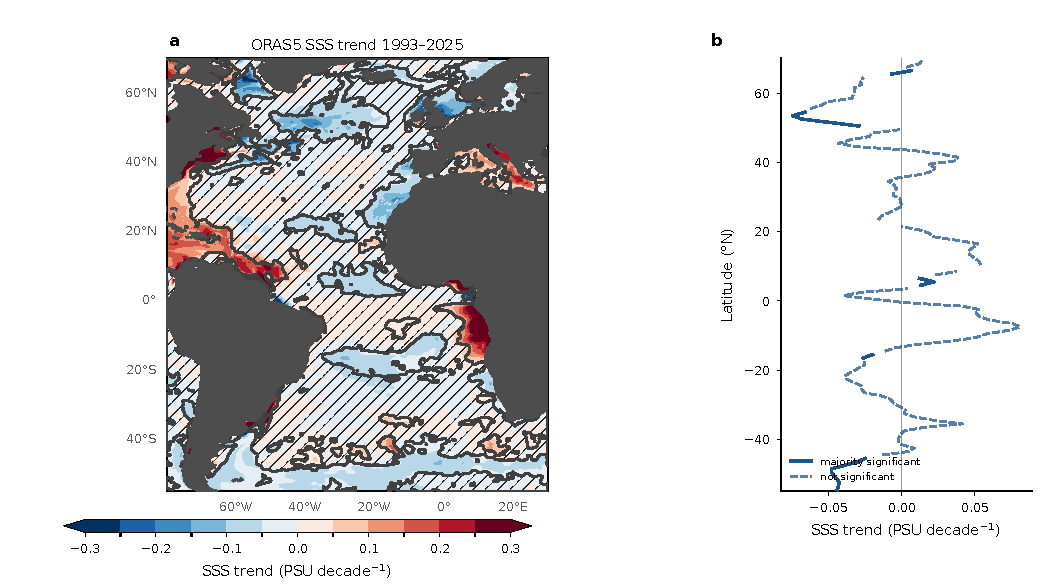
\includegraphics[width=0.94\textwidth]{../extended_data/ED1a_sss_trend_oras5.pdf}\\[0.4em]
  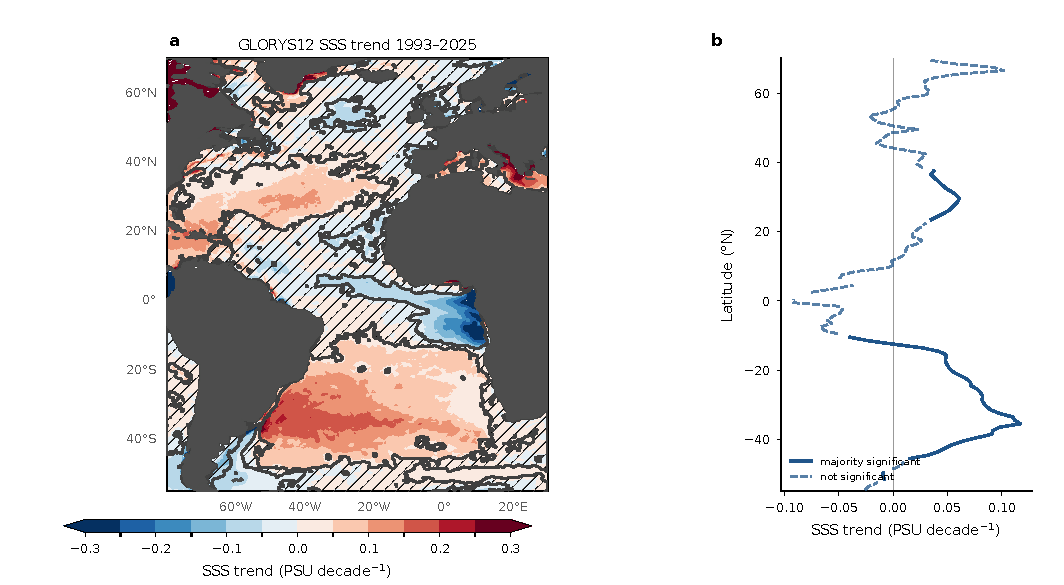
\includegraphics[width=0.94\textwidth]{../extended_data/ED1b_sss_trend_glorys12.pdf}
  \caption*{}
\end{figure}

\textbf{Extended Data Fig.~1 $\vert$ Surface salinity trends, 1993--2025.}
Per-pixel trends on deseasonalised monthly anomalies for ORAS5 and GLORYS12V1,
hatched where the Santer-adjusted $p$ exceeds 0.05. The effective-sample-size
correction reduces the significant ocean area from 76\% to 36\% in ORAS5 and
from 76\% to 51\% in GLORYS12V1. Atlantic band means disagree in sign between
the products in all three bands examined (60\degN{} to 80\degN{}, 40\degN{} to
60\degN{}, 10\degS{} to 35\degS{}), and only one of the six band-and-product
combinations is significant, GLORYS12V1 over 10\degS{} to 35\degS{}
($+0.061$~PSU per decade, $p=0.0002$). There is no significant subpolar North
Atlantic freshening in either product. Surface salinity trend patterns are in
any case ambiguous, since amplification of the water cycle and a uniform surface
heat flux both produce patterns resembling the one that would be attributed to
ocean transport\cite{Zika2018}, which is why the argument in the main text rests
on the transport-weighted limb salinities at the section and these maps are not
used as evidence.

\begin{figure}[h]
  \centering
  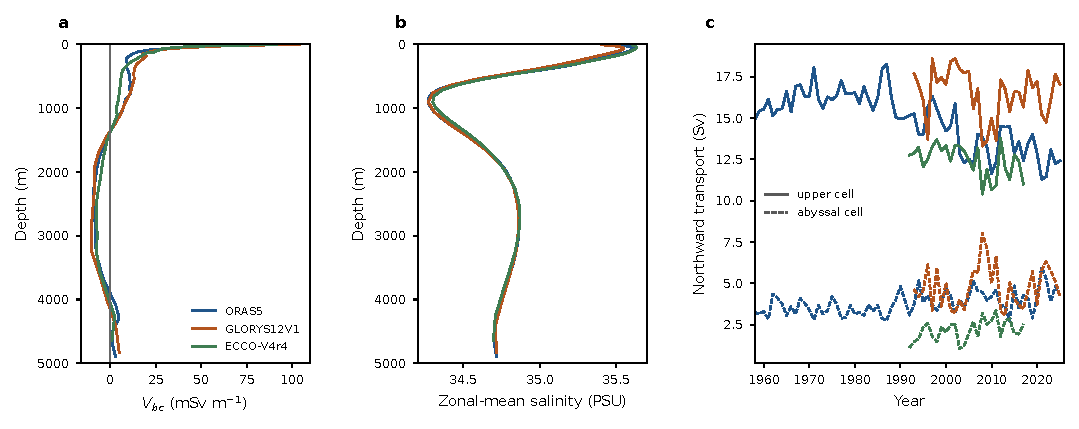
\includegraphics[width=0.98\textwidth]{../extended_data/ED2_section.pdf}
  \caption*{}
\end{figure}

\textbf{Extended Data Fig.~2 $\vert$ Section profiles and the structure of the
limbs.} \textbf{a}, Time-mean zonally integrated meridional velocity after
removal of the net section transport, over the matched 1993--2017 window. The
sign changes of this profile define the limbs. \textbf{b}, Time-mean zonally
averaged salinity over the same window. \textbf{c}, The northward-limb transport
split into its upper cell (solid) and its abyssal cell (dashed), on monthly
fields so that the two sum to $T$. The barotropic-corrected velocity changes sign
three to seven times in ORAS5 (modally four), three to four in GLORYS12V1 and
three to five in ECCO; the upper limb reaches to about 1325, 1245 and 1318~m
respectively, and the abyssal limb begins at about 4044, 4405 and 4264~m. The abyssal cell carries 3.8, 4.8 and 2.2~Sv, that is 20\%,
23\% and 15\% of the northward limb, and is 0.21 to 0.49~PSU fresher than the
upper cell, which is why the redistribution between them has to be excluded
before the widening contrast can be read as a water-mass change. Its transport trend
is significant in ECCO ($+0.36$~Sv per decade, $p=0.041$) and in ORAS5
($+0.17$, $p=0.0004$), and not in GLORYS12V1.

\textbf{Extended Data Table~1 $\vert$ Reanalysis products.}

\begin{center}
\small
\begin{tabular}{lllll}
\toprule
 & ORAS5 & GLORYS12V1 & ECCO-V4r4 & SODA 3.15.2 \\
\midrule
Ocean model        & NEMO & NEMO & MITgcm & MOM5, SIS \\
Model resolution   & 0.25$^\circ$ & 1/12$^\circ$ & LLC90, $\sim$1$^\circ$ & 0.25$^\circ$ \\
Grid analysed      & native & native & 0.5$^\circ$ lat-lon & 0.5$^\circ$ Mercator \\
Vertical levels    & 75 & 50 & 50 & 50 \\
Assimilation       & NEMOVAR 3D-Var & reduced-order & adjoint & optimal \\
                   & FGAT           & Kalman filter & (no increments) & interpolation \\
Atmospheric forcing & ERA-40, ERA-Interim, & ERA-Interim, & ERA-Interim & ERA5 \\
                    & ERA5 & ERA5 & (adjusted) & (COARE4) \\
Fields used        & 816 monthly & 396 monthly & 312 monthly & 43 annual \\
$T$, 1993--2017 (Sv) & 17.9 & 21.1 & 14.6 & not recomputed \\
Record             & 1958--2025 & 1993--2025 & 1992--2017 & 1980--2022 \\
Ocean points       & 294 & 881 & 146 & not recomputed \\
$T$ (Sv)           & 18.7 & 21.3 & 14.6 & not recomputed \\
$\Delta S$ (PSU)   & $+0.068$ & $+0.136$ & $+0.307$ & not recomputed \\
Used quantitatively & yes & yes & yes & no \\
\bottomrule
\end{tabular}
\end{center}
